\section{Introdução}
\label{s.introduction}

\begin{frame}{Introdução}
	\begin{itemize}
		\justifying
		\item Avanços em \textbf{técnicas inteligentes} possibilitaram a resolução de problemas com um mínimo de esforço humano~\cite{Lu:19};
		\\~\\
		\item A área da Inteligência Artificial, do inglês \emph{Artificial Intelligence} (AI), objetiva estudar operações dentro do contexto biológico, tentando \textbf{simular} o funcionamento do \textbf{cérebro} humano~\cite{Bishop:95}.
	\end{itemize}
\end{frame}

\begin{frame}
	\begin{figure}
		\centering
		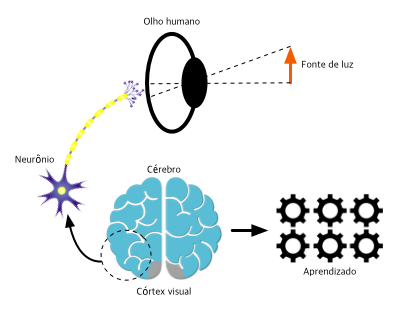
\includegraphics[scale=0.5]{figs/visual_learning.png}	
		\caption{Procedimento simplificado do aprendizado humano através do córtex visual.}
		\label{f.visual_learning}
	\end{figure}
\end{frame}

\begin{frame}
	\justifying
	A área da \textbf{Inteligência Artificial} é demasiada grande e costuma ser \textbf{dividida} em \textbf{subáreas}, por exemplo:
	\\~\\
	\begin{itemize}
		\justifying
		\item Visão Computacional (\emph{Computer Vision});
		\\~\\
		\item Processamento de Linguagem Natural (\emph{Natural Language Processing});
		\\~\\
		\item Aprendizado de Máquina (\emph{Machine Learning});
		\\~\\
		\item Aprendizado em Profundidade (\emph{Deep Learning}).	
	\end{itemize}
\end{frame}

\begin{frame}
	\begin{figure}[!ht]
		\centering
		\includegraphics[scale=0.4]{figs/venn_diagram.eps}	
		\label{f.venn_diagram}
		\caption{Diagrama de Venn entre as áreas de Inteligência Artificial e Ciência de Dados.}
	\end{figure}
\end{frame}